\documentclass[11pt]{article}
\usepackage[final]{acl}
\usepackage{times}
\usepackage{latexsym}
\usepackage[T1]{fontenc}
\usepackage[utf8]{inputenc}
\usepackage{microtype}
\usepackage{booktabs}
\usepackage{graphicx}

\title{Where Did It Go Wrong? Turn-Position Sensitivity of LLM Judges in Multi-Turn Task-Oriented Dialogue}
\author{Sreehari Nair \and Yu-Chiao Chao \and Shreyas Arisa \and Shourya Adluri \\
  \normalfont CS 6604 Final Project Milestone \\
  \normalfont November 21, 2026 \\
  \normalfont\textbf{Preliminary overnight results pending team review}}

\begin{document}
\maketitle

\begin{abstract}
We study how the position of a factual contradiction in a task-oriented dialogue affects detection and scoring by an LLM judge. An initial feasibility pilot exposed factual false alarms and placement cues. In a follow-up using local Qwen3.5-9B, we ran a 36-transcript pilot and evaluated 1,000 edits with matched correct versions from 40 constructed MultiWOZ-based scenarios. The whole-dialogue judge flagged the edited turn in 652 cases, and the turn-by-turn judge flagged it in 945. Whole-dialogue flags rose from 75 of 200 early edits to 189 of 200 late edits. These counts are preliminary and await independent team review of the cases and judge evidence.
\end{abstract}

\section{Introduction}

Task-oriented assistants carry user constraints across multiple turns. For example, a travel assistant can correctly identify the requested departure city at first and name another city later. A judge that scores the full conversation must connect the later claim to the original request, identify the error, and decide how much it affects the dialogue score. An overall score can obscure whether the judge found the underlying error.

We ask three questions. First, does the position of a factual error affect its detection rate? Second, how much does the dialogue score change when the judge identifies the error? Third, does scoring individual replies with dialogue history or explicit state tracking change detection across positions? We hypothesize that a full-transcript judge detects fewer errors in the middle. The initial pilot tests the evaluation pipeline. The overnight run explores how the two judging protocols behave when evidence and reply move together.

\section{Background}

\citet{zheng2023judge} used LLMs to evaluate chat assistants and documented sensitivity to the order in which candidate responses are presented. \citet{shi2025judging} studied that order effect systematically. In our experiment, position refers to the chronological location of a flaw inside one transcript. \citet{liu2024lost} found that models often retrieve evidence less effectively when it appears near the middle of a long context. Their retrieval and question-answering results motivate our hypothesis about transcript grading.

Prior work also examines flaws within conversations. \citet{ivry2026lalm} study the position of a localized unsafe turn in spoken dialogues, including a text-only judging condition. \citet{tang2026rankjudge} generate dialogue pairs with labeled flaws and measure whether judges identify the worse conversation, the flawed turn, and the type of failure. Our experiment focuses on factual contradictions in task-oriented dialogue and measures error detection separately from dialogue scores.

\citet{bai2024mtbench} score individual assistant responses with their preceding history and take the lowest score as the dialogue grade. \citet{acikgoz2025tdeval} combine context-aware turn judgments with dialogue-level comparisons in task-oriented evaluation. These methods motivate our turnwise baselines. We use MultiWOZ 2.4 because its revised validation and test annotations support later analysis of dialogue-state tracking \citep{ye2022multiwoz}.

\section{Initial feasibility pilot}

\paragraph{Data and edit.}
We define an assistant turn as one assistant response. For the initial feasibility pilot, we selected three dialogues from the 171 MultiWOZ 2.4 test dialogues with at least ten assistant responses.

Each pilot dialogue begins with a user specifying a train route. For each base dialogue, we append the same false departure or destination claim to exactly one assistant response in each of five variants. The target positions are the first response, responses nearest to 25\%, 50\%, and 75\% of the interval between the first and last responses, and the last response. The 15 edited transcripts each have an untouched counterpart among the three originals. All other turns stay identical. The user constraint is present before every edit, allowing the judge to identify the contradiction from the transcript.

\paragraph{Judges.}
The holistic baseline, J1, receives the complete transcript, assigns an integer score from 1 to 10, and lists up to three issues with turn numbers and explanations. J3 adapts the MT-Bench-101 minimum-turn method to task-oriented dialogue. Each call scores one assistant response and can flag an issue, with history available through that response. The dialogue score is the minimum over replies. Both protocols receive dialogue text only and use the same underlying model.

\paragraph{Measures.}
Under the pilot labeling rule, a detection flags the incorrect route claim at the edited turn. This rule allows a detection alongside a flawed justification. The paired score drop is the original score minus the edited score, with negative values indicating an increase after editing. We checked selected factual criticisms of the originals against the bundled train and restaurant records and distinguished database-verified false alarms from genuine issues already present in the original.

\paragraph{Reproducibility.}
The preparation script stores the base dialogue identifier, edit position, expected turn, and exact transcript for each case. Inference uses the saved prompt for each protocol and the same model and sampling settings across positions. The run logs store responses alongside parsed scores and issue descriptions, model settings, and hashes of the prompt and input cases. An identical dialogue prefix can share a deterministic J3 completion. We retain the resulting turn evaluations within each variant and distinguish reused evaluations from inference requests.

\section{Preliminary baseline results}

In initial prompt calibration, local Qwen3.5-0.8B assigned 9/10 and an empty issue list to all 18 pilot transcripts. The response-format example contained the score 9. After we removed the numeric example, this model flagged three injected claims and assigned 8/10 to every transcript.

We then ran J1 and J3 locally using the same Qwen3.5-9B model (Q4\_K\_M quantization) in llama.cpp, with thinking disabled and temperature zero. Under the pilot labeling rule, both protocols flagged the injected route error in all 15 variants. J1 lowered the score in five cases, left it unchanged in seven, and raised it in three. All five decreases came from the one original that J1 scored 9/10. The other two originals each scored 2/10, leaving only one point of downward room.

J3 gave all 15 edited dialogues a lower minimum score than their originals, and 14 reached the 1/10 floor. Across positions, the mean drops ranged from 6.00 to 6.33 points for J3 and from $-0.33$ to 2.33 for J1 (Figure~\ref{fig:positions}). J1 took 18 inference requests. J3 produced 186 turn scores from 114 distinct transcript prefixes, reusing outputs for identical inputs.

\paragraph{Aggregation sensitivity.}
Across all 15 pairs, the mean score drop was 6.27 points when we took the minimum turn score. Taking the mean over the same saved turn scores yielded a 2.32-point drop. Both aggregations gave a lower score to all 15 edited dialogues. The choice of rule therefore changed the size of the penalty even with identical turn judgments. In the Norwich 75\% variant, J3 gave the edited reply 2/10. The dialogue minimum of 1/10 came from a later, untouched reply because the judge revisited the restaurant details.

\paragraph{Audit of original judgments.}
The judges saw transcript text only. We checked three factual criticisms against the archived MultiWOZ records. In the Cambridge-to-Peterborough original (PMUL1801), J1 caught the typo \textit{Gald} and questioned the fare. The bundled record for train TR1086 gives \pounds13.20 per ticket, which verifies the quoted \pounds92.40 for seven. J1 flagged the Ely substitution in the early edit and gave both versions 2/10.

In the Norwich-to-Cambridge original (PMUL0509), the address and phone match Frankie and Bennys record 19195. J1 gave the dialogue 2/10 and reported an alleged mismatch as its sole issue. In the London-to-Cambridge original (MUL1569), the restaurant database has no South Indian entry. J3 nonetheless gave the reply reporting this result 2/10 and the other ten replies 10/10. The mistaken 2/10 set the dialogue score. Pre-existing flaws, factual false alarms, and scoring headroom all influence the paired scores.

\begin{figure}[t]
  \centering
  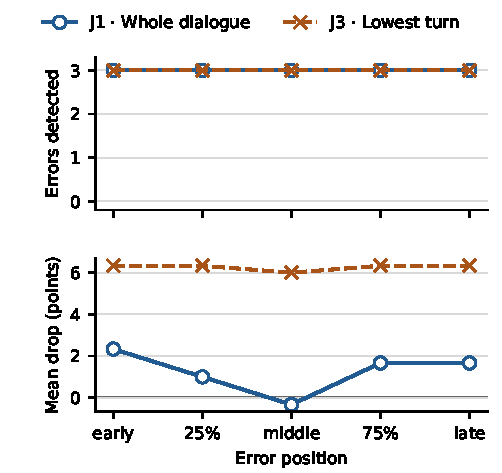
\includegraphics[width=\columnwidth]{position-curve.pdf}
  \caption{Qwen3.5-9B feasibility pilot across five assistant reply positions, with three edited dialogues per position. Detection uses the original pilot labeling rule. Score drops are paired differences from the unedited counterparts on the 1--10 scale.}
  \label{fig:positions}
\end{figure}

\subsection{Correct-route placement controls}

We tested whether the appended sentence could attract criticism even when the route was correct. For each of the 15 route-error variants, we kept the sentence in the same reply and replaced only Ely with the correct requested location. These controls preserve the placement and phrasing of the appended claim. Place names can differ in length. We reran J1 with the same prompt, model and decoding settings on the 15 counterparts using the local model. All 15 returned valid judgments.

We coded a placement flag when the explanation explicitly criticized the appended claim's timing, repetition or relevance. We coded a route challenge when the explanation called the correct location wrong or unsupported. Both tallies are specific to the appended claim and can overlap.

\begin{table}[ht]
  \centering
  \begin{tabular}{lrr}
    \toprule
    Position & Placement flags & Route challenges \\
    \midrule
    Early & 0 & 0 \\
    25\% & 1 & 0 \\
    Middle & 0 & 0 \\
    75\% & 1 & 0 \\
    Late & 2 & 2 \\
    \midrule
    Total & 4 & 2 \\
    \bottomrule
  \end{tabular}
  \caption{J1 flags on the correct-route controls. Each position has three variants. One late route challenge is ambiguous because the explanation also acknowledges the correct destination and ends mid-sentence.}
  \label{tab:route-controls}
\end{table}

J1 flagged placement in four controls, including two closing turns (Table~\ref{tab:route-controls}). In the late Norwich control, J1 correctly recognized that the train task was over and called the requested departure city a hallucination. In the late Peterborough control, J1 called the destination statement incorrect, then acknowledged that the user had requested Peterborough. We count that response as an explicit challenge and treat its rationale as ambiguous.

Relative to these matched correct-route controls, false-route copies scored lower in six pairs, tied in seven, and scored higher in two. The correct-route controls themselves tied the untouched originals in 13 pairs, scored lower in one, and scored higher in one. These comparisons show that J1 can object to the placement of a factual statement and can raise a factual concern about a correct one. With three base dialogues, the controls illustrate the confound and motivate the redesigned pilot.


\section{Changes since the proposal}

The proposal targets 40 base dialogues, five error types, five positions, and five judging setups. We started with one error type and two protocols to audit the pipeline. The initial append-based edits varied in topic fit and distance from their evidence. For example, the Peterborough claim is immediately adjacent to Ely in the 25\% variant, while the late variant appends Ely to a goodbye. The correct-route controls show that the placement itself could draw criticism. The overnight design moves the request and readback together and uses a matched correct version at every position.

\section{Overnight Qwen results (preliminary)}
\label{sec:overnight}

\paragraph{Constructed test cases.}
The overnight run used train-search requirements from MultiWOZ 2.4 test goals. We constructed each 12-reply dialogue around a two-exchange readback block and four independent travel-related blocks. Within a scenario, the readback block moves while the wording and order of the other blocks stay fixed. A correct and an incorrect transcript at each position differ in exactly one readback value. The user states the supporting requirement one exchange before the readback in every variant. Some party sizes were constructed where the source goal lacked one.

We ran a 36-transcript pilot from six source goals, covering destination and day errors at three positions. The full batch used 40 separate source goals, each crossed with five errors (departure, destination, day, time cutoff, and party size) at five positions (assistant replies 3, 5, 7, 9, and 11). This yielded 1,000 edited transcripts and 1,000 paired correct versions. The five errors at a given source and position share the same correct transcript, yielding 200 distinct correct versions.

\paragraph{Judging and detection.}
We ran Qwen3.5-9B locally on a Mac using llama.cpp, with Q4\_K\_M quantization, thinking disabled, temperature zero, and \$0 in API spend. J1 reviewed the whole dialogue and could return one issue per reply. J3 reviewed each reply with its preceding history and used the minimum turn score for the dialogue. An issue recorded the assistant reply, supporting user turn, observed value, and expected value. A raw flag is any issue recorded at the edited reply. The stricter automated match also requires the recorded supporting user turn and both values to match the case metadata after normalization. This check can miss correct phrases that include extra words.

\begin{table}[t]
  \centering
  \begin{tabular}{lrr}
    \toprule
    Readback position & J1 & J3 \\
    \midrule
    Early & 75 & 186 \\
    25\% & 109 & 193 \\
    Middle & 124 & 187 \\
    75\% & 155 & 189 \\
    Late & 189 & 190 \\
    \midrule
    Total & 652 & 945 \\
    \bottomrule
  \end{tabular}
  \caption{Raw edited-reply flags in the preliminary full batch. Each position contains 200 edits.}
  \label{tab:overnight-flags}
\end{table}

\paragraph{Results.}
In the 18 pilot pairs, J1 flagged 11 edited replies and J3 flagged 18. Strict matches totaled 3 and 9, respectively. The full batch yielded 2,000 J1 dialogue judgments and 24,000 J3 turn judgments, with reuse for identical inputs. J1 flagged 652 edited replies and J3 flagged 945 (Table~\ref{tab:overnight-flags}). Strict matches totaled 142 and 232. Both judges recorded zero target-reply flags on the 1,000 paired correct versions. Relative to the matched correct cases, dialogue scores fell in 652 J1 pairs and 947 J3 pairs, with mean decreases of 3.44 and 7.42 points on the 1--10 scale. J3 recorded 2,083 flags after the edited reply across 784 edited cases, and its minimum fell below the edited reply's score in 59 cases. These later flags require review because only the readback was changed.

\paragraph{Interpretation.}
J1 flagged more edits at later positions in this batch, while J3 flags varied less by position. The protocols have different input scopes, and the transcripts share templates and source goals. The 1,000 edits therefore represent repeated comparisons within 40 source goals. Treat these results as descriptive pending blinded team review of the cases and cited evidence. Analyze uncertainty at the source-goal level after review, and test whether the pattern extends to naturally occurring dialogues.


\section{Remaining work}

\begin{itemize}
  \item \textbf{Nov. 21--24.} Ask two teammates to independently review the 18 pilot pairs using the blinded packet. Adjudicate transcript naturalness, the single intended violation, and comparable evidence and consequences across placements. Review judge outputs after agreeing on the reference labels.
  \item \textbf{Nov. 25--30.} Freeze the detection rubric, audit cases across all five error types and positions, and verify evidence for misses, partial hits, and control flags. Select the planned middle-versus-ends comparison before confirmatory evaluation and resample at the base-scenario level. Add the constraint rubric, TD-EVAL adaptation, and state-tracking judge as compute permits.
  \item \textbf{Dec. 1--8.} Reproduce the tables and figures from saved logs, analyze error types and judge behavior, and present the poster on Dec. 3. Incorporate feedback into the final report and code by Dec. 8.
\end{itemize}

\section*{Acknowledgements}
The proposal disclosed using Claude and Gemini for brainstorming. Codex assisted with code, audit checks, and drafting this milestone.

\clearpage
\bibliography{references}

\end{document}
